  %2017-09-20
  \subsection{Плоскопараллельное движение}
  \begin{df}
  Движение твердого тела называется плоскопараллельным, если скорости всех точек тела параллельны некоторой неподвижной плоскости:
  $$ \v{v}_{p_i} \parallel \pi,~ \forall p_i \in \text{АТТ} $$
  \end{df}

  $$ \v{v}_{p_i} = \v{v}_{p_j} + [\v{\omega}, \v{p_j p_i}] $$
  $$ 
  (\v{p}_i - \v{v}_{p_i}) = 0 \Leftrightarrow 
  \left[
  \begin{array}{l}
  \v{\omega} = 0 \\
  \v{v}_{p_i} = \v{v}_{p_j},~ \forall p_i, p_j \in \text{АТТ} \\
  \v{\omega} \perp \v{p}_i - \v{v}_{p_i} \parallel \pi \\
  \end{array}
  \right.
  $$
  $$ \v{v}_{M_i} = \v{v}_{M_j} + \omega [\v{\omega}, \overline{M_jM_i}] = \v{v}_{M_j},~~ \forall M_i, M_j: \overline{M_iM_j} \perp \pi \Rightarrow \v{w}_{M_i} = \v{w}_{M_j} $$
  Качение:
  $$ \v{r}_S = x_S \v{e}_x + y_S \v{e}_y $$
  $$ \dot{\v{e}}_{\xi} = \dot{\varphi}\v{e}_{\eta},~~ \dot{\v{e}}_{\eta} = \dot{\varphi}\v{e}_{\zeta},~~ \dot{\v{e}}_{\zeta} = 0$$
  $$ \v{\omega} = \dot{\varphi} \v{e}_z,~~ \v{\varepsilon} = \ddot{\varphi} \v{e}_z \parallel \v{\omega}$$
  $$ \v{v}_M = \v{v}_S + [\v{\omega}, \overline{SM}] $$
  $$ \v{w}_M = \v{w}_S + [\v{\varepsilon}, \overline{SM}] + [\v{\omega}, [\v{\omega}, \overline{SM}]] = \v{w}_s + [\v{\varepsilon}, \overline{SM}] - \omega^2 \overline{SM} $$ 

  \begin{teo}
  Если при плоскопараллельном движении угловая скорость твердого тела отлична от нуля, то существует точка, скорость которой равна нулю в данный момент времени.
  \end{teo}
  \begin{proof}
  $$
  \begin{cases}
  \v{v}_c = \v{v}_s + [\v{\omega}, \v{SC}] \\
  \v{v}_c = 0 \\
  \end{cases}
  \Rightarrow
  [\v{\omega}, \v{v}_s] + [\v{\omega}, [\v{\omega}, \v{SC}]] = 0 $$
  $$ [\v{\omega}, \v{v}_s] + \v{\omega}(\v{\omega}, \v{SC}) - \omega^2 \v{SC} = 0 $$
  $$ \v{SC} = \frac{[\v{\omega}, \v{v}_s]}{\omega^2} $$
  \end{proof}
  \begin{cor} 
  Любое плоскопараллельное движение является либо мгновенно-поступательным, либо мгновенно-вращательным
  \end{cor}
  \begin{proof}
  $\v{\omega} = 0$ - мгновенно-поступательное. $\v{\omega}(t) \neq 0$ - вращение вокруг $l$. 
  
  \end{proof}

  \begin{figure}[H]
  \centering
  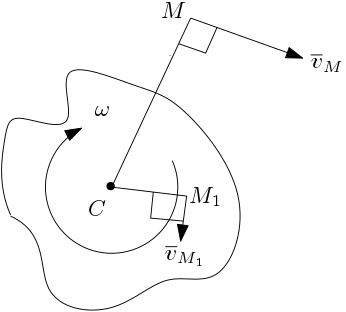
\includegraphics[width=5cm]{fig8.png} 
  \end{figure}  

  \begin{df}
  $C$ - мгновенный центр скоростей
  \end{df}
  \begin{ntc}
  Положение $C$ меняется со временем.
  \end{ntc}
  \begin{xmp}
  Качение без проскальзывания
  \end{xmp}

  \subsection{Тело с неподвижной точкой (вращение вокруг точки)}
  $$ \exists \v{v}_0 \equiv 0 $$
  $$ l \parallel \v{\omega}, O \in l $$
  $$ \v{v}_M = \v{v}_0 + [\v{\omega}, \v{OM}] = 0 + 0,~ \forall M \in l $$
  \begin{figure}[H]
  \centering
  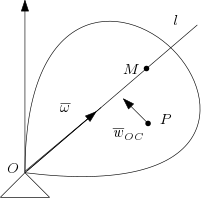
\includegraphics[width=5cm]{fig9.png} 
  \end{figure}  

  \begin{df} 
  $l$ - мгновенная ось вращения 
  \end{df}
  $$ \v{v}_p = [\v{\omega}, \v{OP}],~ \v{w_p} = [\v{\varepsilon}, \v{OP}] + \underbrace{[\v{\omega}, [ \v{\omega}, \overline{OP}]]}_{\v{v}_{OC}} $$
  \subsection{Винтовое движение}
  \begin{df} 
  Движение твердого тела называется винтовым, если тело равномерно вращается вокруг неподвижной оси, а скорости всех точек, лежащий на этой оси, равны между собой, постоянны и сонаправлены с осью.
  \end{df}
  \subsection{Общий случай}
  \begin{teo}
  $ \v{\omega} \neq 0 \Rightarrow \exists l:~ \v{\omega} \parallel l,~ \v{v}_{k_i} \parallel l,~ \forall k_i \in l$
  \end{teo}
  \begin{figure}[H]
  \centering
  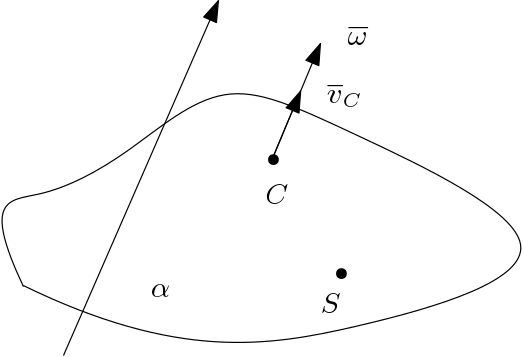
\includegraphics[width=5cm]{fig10.png} 
  \end{figure}  

  \begin{proof}
  $$ \v{\alpha} \perp \v{\omega},~ S \in \alpha $$
  $$
  \begin{cases}
  \v{v}_c = \v{v}_c = \v{v}_s + [\v{\omega}, \v{SC}] \\
  \v{v}_c = \lambda \v{\omega}
  \end{cases}
  \Rightarrow
  0 = [\v{\omega}, \v{v}_s] + [\v{\omega}, [\v{\omega}, \v{SC}]]
  $$
  $$ [ \v{\omega}, \v{v}_s] + \v{\omega}(\v{\omega}, \v{SC}) - \omega^2 \v{SC} = 0 $$
  $$ \v{SC} = \frac{[\v{\omega},\v{v}_c]}{\omega^2} $$
  $$ \exists l: C \in l, l \parallel \v{\omega} $$
  $$ \v{v}_{C_1} = \v{v}_C + [\v{\omega}, \v{CC_1}] = \v{v}_C,~~ \forall C_1 \in l$$ 

  \end{proof}
  $$\v{v}_C = \v{v}_S + \left[ \v{\omega}, \frac{[\v{\omega}, \v{v}_C]}{\omega^2} \right] = \v{v}_S + \frac{1}{\omega^2}\left(\v{\omega}(\v{\omega}, \v{v}_S) - \omega^2\v{v}_S \right) = \underbrace{\frac{(\v{\omega}, \v{v}_S)}{\omega^2}}_{\lambda} \v{\omega}$$
  $$\lambda = \frac{(\v{\omega}, \v{v}_S)}{\omega^2} \text{ - параметр (шаг винта).}$$

  \begin{cor}
  Любое движение твердого тела является в каждый момент времени либо мгновенно-поступательным ($\omega = 0$, $\lambda \rightarrow +\infty$), либо мгновенно-вращательным ($\omega \neq 0$, $\lambda = 0$) , либо мгновенно-винтовым ($\omega \neq 0$, $\lambda \neq 0$).
  \end{cor}
  \begin{df}
  $\{l, \v{\omega}, \v{v}\}$ - кинематический винт.
  \end{df}
  $$\v{v}_S = v_x\v{e}_x + v_y\v{e}_y + v_z\v{e}_z$$
  $$\v{r}_S = x_S\v{e}_x + y_S\v{e}_y + z_S\v{e}_z$$
  $$\v{\omega} = \omega_x\v{e}_x + \omega_y\v{e}_y + \omega_z\v{e}_z$$
  $$ \v{r}_C = x\v{e}_x + y\v{e}_y + z\v{e}_z $$
  $$ \v{v}_S + [\v{\omega}, \v{SC}] = \lambda \v{\omega} \Rightarrow \lambda = \frac{v_x + \omega_y(z - z_S) - \omega_z(y - y_S)}{\omega_x} = $$
  $$ = \frac{v_y + \omega_z(x - x_S) - \omega_x(z - z_S)}{\omega_y} = \frac{v_z + \omega_x(y - y_S) - \omega_y(x - x_S)}{\omega_z} $$
  

  \section{Кинематика сложного движения}
  \begin{figure}[H]
  \centering
  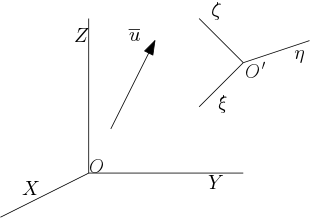
\includegraphics[width=5cm]{fig11.png} 
  \end{figure}  

  $OXYZ$ - неподвижная система отсчета ($\v{r})$, $O_1\xi\eta\zeta$ - подвижная система отсчета ($\v{\rho}$).

  $$ \v{u} = u_x \v{e}_x + u_y \v{e}_y + u_z \v{e}_z $$
  $$ \v{u} = u_{\xi} \v{e}_{\xi} + u_{\eta} \v{e}_{\eta} + u_{\zeta} \v{e}_{\zeta} $$
  $$ \frac{d\v{u}}{dt} = \dot {u_x} \v{e}_x + \dot{u_y} \v{e}_y + \dot{u_z} \v{e}_z \text{ - абсолютная производная} $$
  $$ \dot{\v u} = \dot{u_{\xi}} \v{e}_{\xi} + \dot{u_{\eta}} \v{e}_{\eta} + \dot{u_{\zeta}} \v{e}_{\zeta} \text{ - относительная производная}$$
  \begin{teo}(Связь абсолютной и относительной производной) 
  $\frac{d\v{u}}{dt} = \dot{\v{u}} + [\v{\omega}, \v{u}]$, где $\v{\omega}$ - угловая скорость $O_1\xi\eta\zeta$ относительно $OXYZ$
  \end{teo}
  \begin{proof}
  $$ \frac{du}{dt} = \dot{u}_{\xi}\v{e}_{\xi} + \dot{u}_{\eta}\v{e}_{\eta} + \dot{u}_{\zeta}\v{e}_{\zeta} + u_{\xi}\frac{d\v{e}_{\xi}}{dt} + u_{\eta}\frac{d\v{e}_{\eta}}{dt} + u_{\zeta}\frac{d\v{e}_{\zeta}}{dt} = $$
  $$ = \dot{\v{u}} + u_{\xi}[\v{\omega}, \v{e}_{\xi}] + u_{\eta}[\v{\omega}, \v{e}_{\eta}] + u_{\zeta}[\v{\omega}, \v{e}_{\zeta}] = \dot{\v{u}} + [\v{\omega}, \v{u}] $$
  $$ \left(\frac{d\v{e}_i}{dt} = [\v{\omega}, \v{e}_i] - \text{ - формула Пуассона},~~ \dot{\v{e}}_i = 0\right) $$
  \end{proof}
  \subsection{Сложное движение материальной точки}
  \begin{figure}[H]
  \centering
  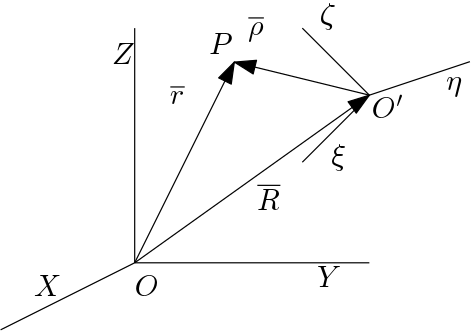
\includegraphics[width=5cm]{fig12.png} 
  \end{figure}
  \begin{df}
  Абсолютной скоростью материальной точки называется ее скорость относительно неподвижной системы отсчета. $\v{v}_{\text{абс}} = \frac{d}{dt}\v{r}$
  \end{df}
  \begin{df}
  Относительной скоростью материальной точки называется ее скорость относительно подвижной системы отсчета. $\v{v}_{\text{отн}} = \dot{\v{\rho}}$
  \end{df}
  \begin{df}
  Переносной скоростью материальной точки называется абсолютная скорость той точки подвижной системы отсчета, в которой находится движующаяся точка в данный момент времени.
  \end{df}
  \begin{teo}
  [Формула сложения скоростей] $\v{v}_{\text{абс}} = \v{v}_{\text{отн}} + \v{v}_{\text{пер}}$
  \end{teo}
  \begin{proof}
  $$ \v{v}_{\text{абс}} = \frac{d}{dt}(\v{R} + \v{\rho}) = \frac{dR}{dt} + \dot{\v{\rho}} + [\v{\omega}, \v{\rho}] = $$
  $$ = \v{v}_{O_1} + \v{v}_{\text{отн}} + [\v{\omega}, \v{\rho}] = \v{v}_{\text{отн}} + \v{v}_{\text{пер}} $$
  \end{proof}
  \begin{df}
  Абсолютным ускорением материальной точки называется ее ускорение относительно неподвижной системы отсчета. $\v{w}_{\text{абс}} = \frac{d}{dt}\v{v}_{\text{абс}}$
  \end{df}
  \begin{df}
  Относительным ускорением материальной точки называется ее ускорение относительно подвижной системы отсчета. $\v{w}_{\text{отн}} = \dot{\v{v}_{\text{отн}}}$
  \end{df}
  \begin{df}
  $ \v{w}_{\text{пер}} = \v{\omega}_{O_1} + [\v{\varepsilon}, \v{\rho}] + [\v{\omega}, [\v{\omega}, \v{\rho}]] $
  \end{df}
  \begin{df}
  $ \v{w}_{\text{кор}} = 2[\v{\omega}, \v{v}_\text{отн}] $
  \end{df}
  \begin{teo}
  [Формула сложения ускорений] $\v{w}_{\text{абс}} = \v{w}_{\text{отн}} + \v{w}_{\text{пер}} + \v{w}_{\text{кор}}$
  \end{teo}

  \begin{proof}
  $$ \v{w}_{\text{абс}} = \frac{d}{dt}(\v{v}_{\text{отн}} + \v{v}_{\text{пер}}) = \frac{d}{dt} (\v{v}_{\text{отн}} + \v{v}_{O_1} + [\v{\omega}, \v{\rho}]) = $$ 
  $$ = \dot{\v{v}}_{\text{отн}} + [\v{\omega}, \v{v}_{\text{отн}}] + \frac{d}{dt}\v{v}_{O_1} + \left[\frac{d\v{\omega}}{dt}, \v{\rho}\right] + [\v{\omega}, \v{\rho} + [\v{\omega}, \v{\rho}]] = $$ 
  $$ = \dot{\v{v}}_{\text{отн}} + \dot{\v{v}}_{O_1} + [\v{\varepsilon}, \v{\rho}] + 2[\v{\omega}, \v{v}_{\text{отн}}] + [\v{\omega}, [\v{\omega}, \v{\rho}]] $$
  \end{proof}